\documentclass{article}

\usepackage[preprint]{tmlr}

\usepackage{amsmath,amssymb,amsfonts}
\usepackage{booktabs}
\usepackage{graphicx}
\usepackage{hyperref}
\usepackage{xcolor}

\renewcommand{\arraystretch}{1.3}
\setlength{\abovetopsep}{6pt}
\graphicspath{{figures/}}

\title{Ollivier-Ricci Curvature Distinguishes Hubs from Bridges in Psychiatric Comorbidity Networks}

\author{\name Elliot Tower \\
      \email elliot@elliottower.ai}

\begin{document}
\maketitle

\begin{abstract}
Network models of psychiatric comorbidity rank disorders by degree or betweenness centrality, treating all edges as structurally equivalent. These metrics cannot distinguish a high-degree hub embedded within a single cluster from a lower-degree node bridging separate clusters.

We apply Ollivier-Ricci curvature (ORC)---which compares neighborhoods via optimal transport---to a 23-node, 39-edge comorbidity network assembled from established clinical associations. Within this curated network, generalized anxiety disorder (GAD) emerges as the primary geometric bridge ($\bar\kappa = -0.143$), while major depressive disorder (MDD)---ranked first by betweenness---has near-zero mean curvature ($\bar\kappa = -0.009$), indicating hub character. A paired bootstrap test confirms the separation: the mean difference $\bar\kappa_{\text{GAD}} - \bar\kappa_{\text{MDD}} = -0.080$ has 95\% CI $[-0.201, +0.038]$, with GAD more negative than MDD in 90\% of 1{,}000 perturbation trials.

This distinction is robust: GAD is the top bridge at all 9 values of the laziness parameter ($\alpha = 0.1$--$0.9$), retains rank~1 in 55\% of trials (top~3 in 83\%), survives all 34 single-edge removals (zero flips), and persists under odds-ratio weighting ($\rho = 0.93$ with unweighted rankings). A node-label permutation test ($p = 0.22$) indicates that curvature gaps of this magnitude are not unusual given the degree-heterogeneous topology, underscoring that the hub-bridge distinction is a descriptive structural decomposition rather than a hypothesis test. ORC correlates less with degree ($r = -0.57$) than Forman-Ricci curvature ($r = -0.67$); among four alternative metrics, only ORC and clustering coefficient distinguish GAD from MDD.

To validate beyond the curated graph, we apply ORC to the 120-node, 756-edge symptom network of Boschloo et al.\ (2015), derived from 34{,}653 NESARC respondents. ORC--degree correlation drops to $\rho = -0.25$ (vs.\ Forman--degree $\rho = -0.96$), and the top bridges are cross-diagnostic-boundary symptoms---confirming at five times the scale that ORC captures transdiagnostic structure beyond degree.

If the bridge interpretation holds, GAD remission should reduce cross-cluster comorbidity (panic-spectrum, neurodevelopmental, trauma) more than MDD remission---a prediction testable in longitudinal cohorts such as the NCS-R or NESARC-III.
\end{abstract}

\section{Introduction}

Over half of individuals with one psychiatric disorder meet criteria for at least one other \citep{kessler2005prevalence}. Network models represent this co-occurrence by placing disorders at nodes and comorbidity associations at edges \citep{borsboom2017network, fried2017mental}, then rank nodes by degree, betweenness centrality, or clustering coefficient.

These metrics treat all edges as structurally equivalent. A disorder with high betweenness could sit at the center of a single tight cluster or could connect two otherwise-disconnected communities. The first configuration is a core symptom; the second, a transdiagnostic gateway. Betweenness assigns identical scores to both.

Ollivier-Ricci curvature (ORC) resolves this ambiguity. For an edge $(u, v)$, ORC compares the neighborhoods of $u$ and $v$ through optimal transport \citep{ollivier2009ricci}: negative curvature marks bottleneck edges whose endpoints have non-overlapping neighborhoods; positive curvature marks within-cluster edges. Aggregating curvature across a node's incident edges produces a single number that distinguishes hubs (high degree, near-zero mean curvature) from bridges (lower degree, negative mean curvature).

ORC has been applied to cancer genomics \citep{sandhu2015graph}, brain connectomes \citep{ni2015ricci}, and financial networks \citep{sandhu2016ricci}. Its application to psychiatric comorbidity has not been evaluated. We apply ORC and Ricci flow community detection to a 23-node comorbidity network, assess robustness through parameter sweeps and edge perturbation, and compare the resulting rankings and communities to standard alternatives.

\paragraph{Contributions.}
\begin{itemize}
\item \textbf{Hub-bridge distinction (\S\ref{sec:hubbridge}).} Mean incident curvature separates GAD ($\bar\kappa = -0.143$, bridge) from MDD ($\bar\kappa = -0.009$, hub), reversing the betweenness ranking. A paired bootstrap test on $\bar\kappa_{\text{GAD}} - \bar\kappa_{\text{MDD}}$ confirms the separation (90\% of trials; \S\ref{sec:robustness}). A comparison against Forman-Ricci curvature, clustering coefficient, and edge betweenness (\S\ref{sec:comparison}) shows that ORC is less degree-driven ($r = -0.57$) than Forman ($r = -0.67$) and captures the distinction through local geometry.
\item \textbf{Hidden bridges (\S\ref{sec:novelty}).} OCD jumps $+16$ ranks (betweenness rank~19 $\to$ curvature rank~3), illustrating what curvature detects that betweenness cannot; this jump is specific to cross-community degree-2 nodes, not an artifact of low degree (\S\ref{sec:degree2}).
\item \textbf{Robustness (\S\ref{sec:robustness}).} GAD is the top bridge at all $\alpha \in \{0.1, \ldots, 0.9\}$, in 55\% of 1{,}000 edge-perturbation trials (top~3 in 83\%), and under all 34 single-edge removals (zero flips). The result extends to OR-weighted edges (\S\ref{sec:weighted}; $\rho = 0.93$ with unweighted). A permutation test ($p = 0.22$) indicates the gap's magnitude is not unusual given the topology, motivating validation on larger networks.
\item \textbf{Community structure (\S\ref{sec:communities}).} Ricci flow and Louvain find 4 communities each (NMI $= 0.58$); Ricci flow resolves peripheral dyads that Louvain absorbs.
\item \textbf{Validation at scale (\S\ref{sec:validation}).} On the 120-node, 756-edge symptom network of \citet{boschloo2015network} (NESARC, $N = 34{,}653$), ORC--degree correlation drops to $\rho = -0.25$ (vs.\ Forman $\rho = -0.96$), and the top bridges are cross-diagnostic symptoms---confirming the hub-bridge decomposition on an empirically derived network five times larger.
\end{itemize}

\section{Curvature on a Comorbidity Network}
\label{sec:curvature}

For an edge $(u, v)$ in graph $G = (V, E)$, define probability measures $\mu_u$ and $\mu_v$ that place mass $\alpha$ on the node and distribute $1 - \alpha$ uniformly across neighbors (the lazy random walk). The Ollivier-Ricci curvature is
\begin{equation}
  \kappa_\alpha(u, v) = 1 - \frac{W_1(\mu_u, \mu_v)}{d(u, v)},
  \label{eq:orc}
\end{equation}
where $W_1$ is the Wasserstein-1 distance under the shortest-path metric \citep{ollivier2009ricci}. We report results at $\alpha = 0.5$ and verify stability across $\alpha \in \{0.1, \ldots, 0.9\}$. Optimal transport is solved with the POT library \citep{flamary2021pot}.

The \emph{mean incident curvature} of a node $v$ is the average curvature across all edges incident to $v$:
\begin{equation}
  \bar\kappa(v) = \frac{1}{\deg(v)} \sum_{u : (u,v) \in E} \kappa(u, v).
  \label{eq:node_curvature}
\end{equation}
Nodes with $\bar\kappa < 0$ sit on predominantly bottleneck edges (bridge character). Nodes with $\bar\kappa \approx 0$ despite high degree connect both bottleneck and within-cluster edges (hub character).

\paragraph{Network construction.} The comorbidity network has 23 nodes (8 primary psychiatric disorders, 15 transdiagnostic features) and 39 edges, each supported by at least one published study documenting the association (Appendix~\ref{app:edgelist}). Density is 0.154, clustering coefficient 0.40, diameter 5.

\paragraph{Edge curvatures.} Twelve of 39 edges (31\%) have negative curvature. The three most negative all involve GAD: MDD--GAD ($\kappa = -0.394$), GAD--panic ($\kappa = -0.375$), and GAD--social anxiety ($\kappa = -0.375$; Table~\ref{tab:curvatures}). Each connects distinct symptom clusters---mood to anxiety, anxiety to panic spectrum, anxiety to avoidance. The most positive edges are tightly coupled pairs: SCZ--psychosis, panic--agoraphobia, and social anxiety--avoidance (all $\kappa = +0.500$).

The network's mean curvature ($\bar\kappa = +0.050$) exceeds both Erd\H{o}s-R\'{e}nyi ($\bar\kappa_{\text{ER}} = -0.019$, $z = 1.76$, $p = 0.025$ one-sided) and configuration-model ($\bar\kappa_{\text{CM}} = -0.018$, $z = 1.96$, $p = 0.022$ one-sided) null distributions (10{,}000 samples each; Appendix~\ref{app:null}). One-sided tests are appropriate because the hypothesis---that curated comorbidity edges should produce more positive curvature than random edges, due to the tightly coupled clinical dyads---is directional. These results are consistent with the curvature structure reflecting specific neighborhood overlaps rather than the degree sequence alone.

\begin{table}[t]
\centering
\caption{Selected edge curvatures ($\alpha = 0.5$). Negative curvature indicates bottleneck edges; positive indicates within-cluster edges. Full edge list with citations in Appendix~\ref{app:edgelist}.}
\label{tab:curvatures}
\begin{tabular}{lrl}
\toprule
Edge & $\kappa$ & Structural role \\
\midrule
MDD -- GAD              & $-0.394$ & Mood--anxiety bridge \\
GAD -- panic            & $-0.375$ & Anxiety--panic bridge \\
GAD -- social anxiety   & $-0.375$ & Anxiety--avoidance bridge \\
SUD -- ADHD             & $-0.278$ & Externalizing--neurodevelop. \\
GAD -- PTSD             & $-0.225$ & Anxiety--trauma bridge \\
MDD -- SCZ              & $-0.135$ & Mood--psychosis bridge \\
\midrule
panic -- agoraphobia    & $+0.500$ & Tightly coupled dyad \\
SCZ -- psychosis        & $+0.500$ & Definitional link \\
social anx.\ -- avoidance & $+0.500$ & Tightly coupled dyad \\
ADHD -- ASD             & $+0.417$ & Neurodevelopmental cluster \\
\bottomrule
\end{tabular}
\end{table}

\begin{figure}[t]
\centering
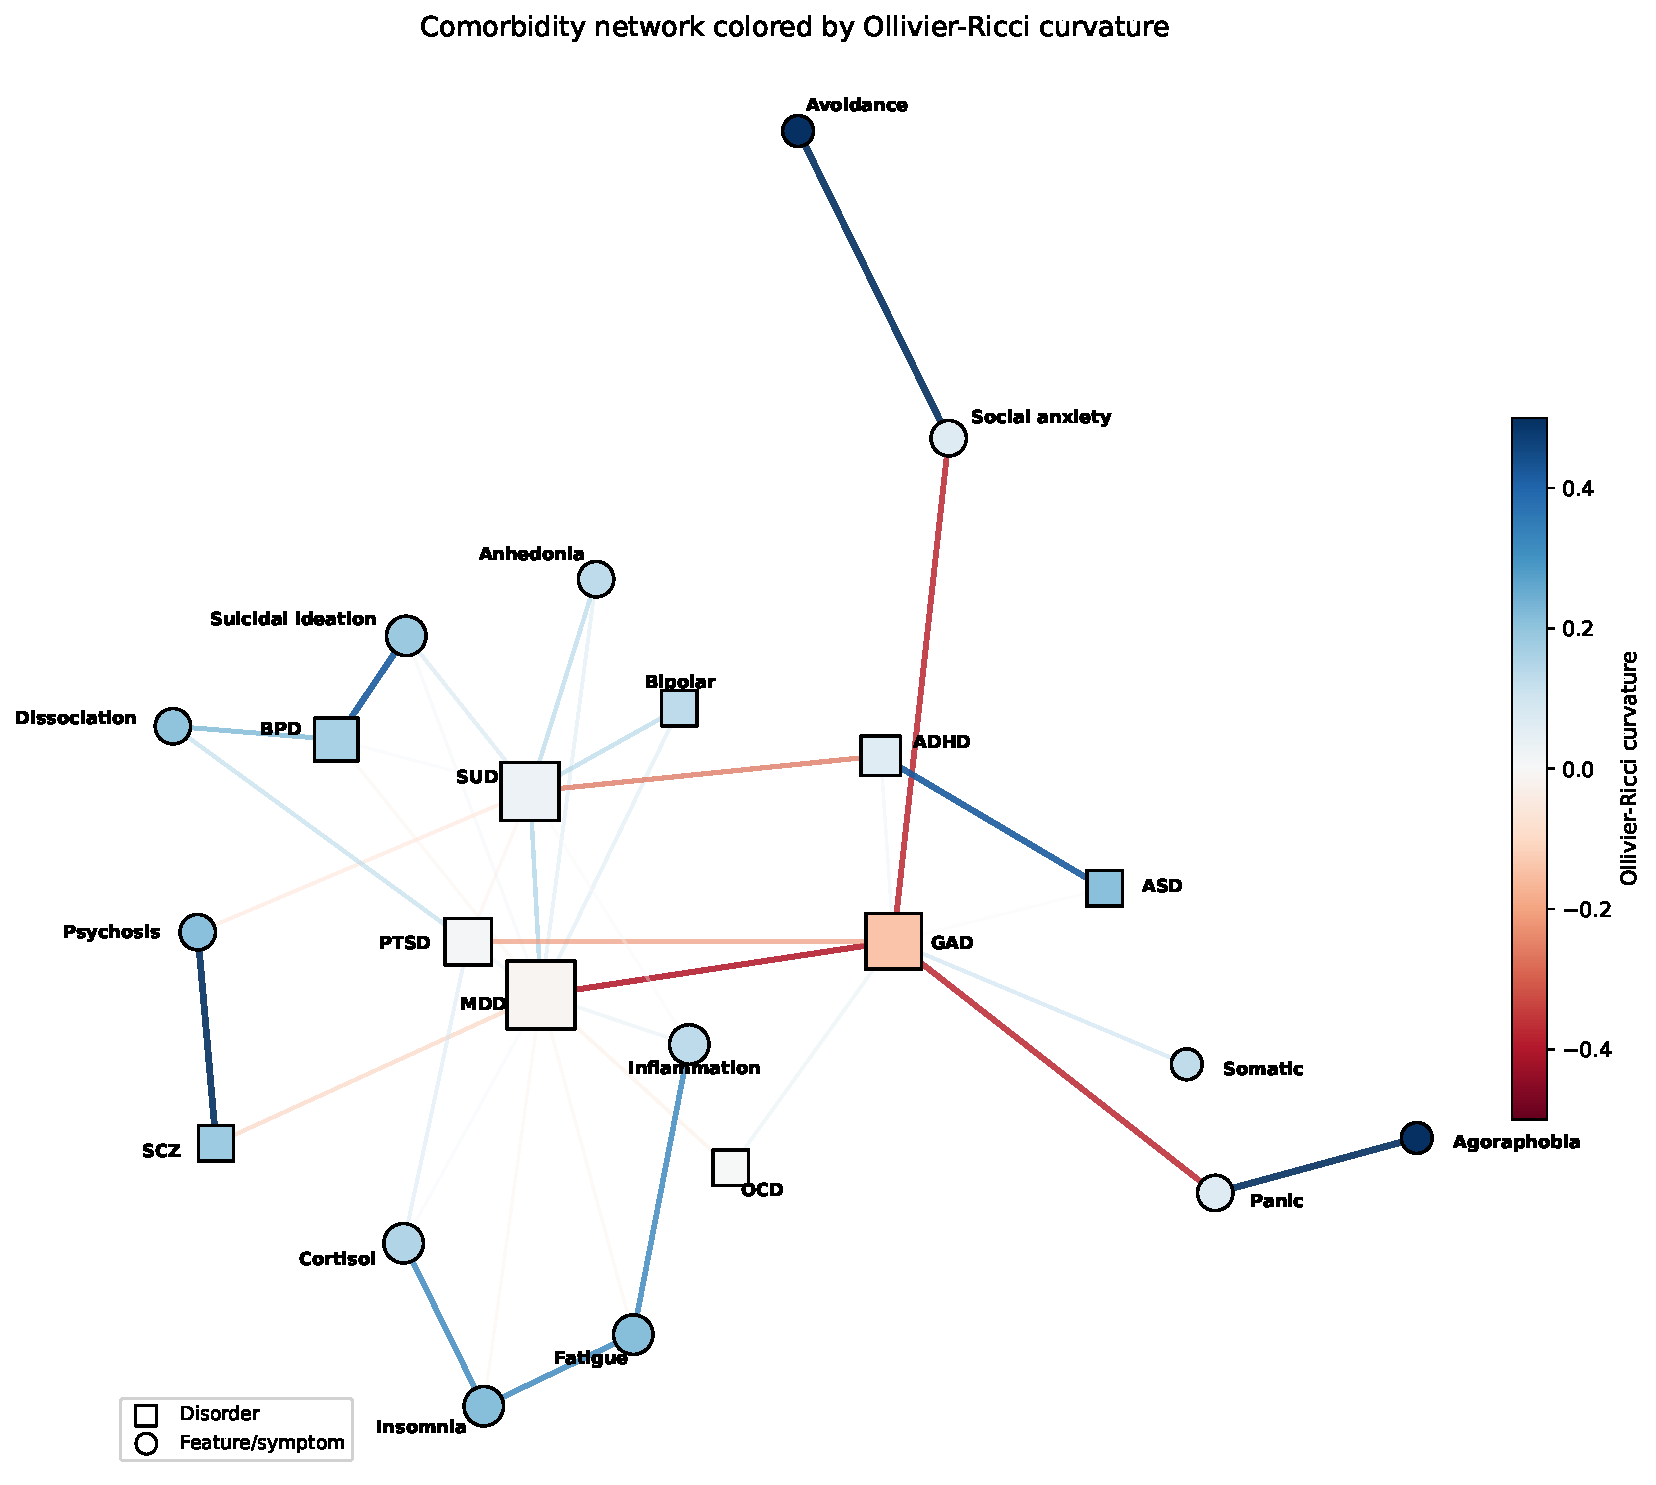
\includegraphics[width=\textwidth]{fig_network.pdf}
\caption{Comorbidity network with edges colored by Ollivier-Ricci curvature (diverging red--blue: red = negative/bottleneck, blue = positive/within-cluster). Node color reflects mean incident curvature $\bar\kappa$; node size scales with degree. Squares are disorders; circles are symptoms/features. The MDD--GAD edge is the deepest red ($\kappa = -0.394$); tightly coupled pairs (SCZ--psychosis, panic--agoraphobia) are deep blue ($\kappa = +0.500$). GAD (salmon, degree~8) sits on predominantly red edges; MDD (near-white, degree~13) has a mix of red and blue.}
\label{fig:network}
\end{figure}

\section{Hubs versus Bridges: GAD and MDD}
\label{sec:hubbridge}

By betweenness centrality, MDD ranks first (0.508) and GAD second (0.469). A standard network analysis would designate MDD as the most structurally important node.

Mean incident curvature reverses this ranking. GAD has $\bar\kappa = -0.143$ (bridge character): its 8 edges are predominantly bottleneck connections between distinct clusters---mood, panic-spectrum, social anxiety, trauma, and neurodevelopmental. MDD has $\bar\kappa = -0.009$ (hub character): its 13 edges span both bottleneck and within-cluster connections, averaging to near-zero (Table~\ref{tab:hubbridge}).

The per-edge distributions clarify the mechanism. GAD's 8 edges include 4 with negative curvature (the most negative: $\kappa = -0.394$, $-0.375$, $-0.375$, $-0.225$) and 3 with weakly positive curvature (max $+0.125$), producing $\bar\kappa = -0.143$ with $\sigma = 0.208$. MDD's 13 edges split 6 negative and 7 positive (range $[-0.394, +0.188]$), averaging to $\bar\kappa = -0.009$ with $\sigma = 0.136$. The difference is that GAD's negative edges are strongly negative while its positive edges are weak; MDD's edges are distributed symmetrically around zero. Both nodes sit on many shortest paths, which is why betweenness ranks them similarly. The difference is that GAD's paths cross community boundaries while MDD's paths run within as well as between communities (Figure~\ref{fig:network}). This distinction---hub versus bridge---is invisible to betweenness, which counts shortest-path participation without regard to the local geometry of each edge.

\begin{table}[t]
\centering
\caption{Hub-bridge distinction for the top-4 nodes by betweenness. GAD has negative mean curvature (bridge); MDD has near-zero (hub).}
\label{tab:hubbridge}
\begin{tabular}{lcccc}
\toprule
Node & Degree & Betweenness & $\bar\kappa$ & Character \\
\midrule
MDD  & 13 & 0.508 & $-0.009$ & hub \\
GAD  &  8 & 0.469 & $-0.143$ & bridge \\
SUD  &  9 & 0.157 & $+0.028$ & hub \\
PTSD &  5 & 0.097 & $+0.011$ & mixed \\
\bottomrule
\end{tabular}
\end{table}

Node removal confirms the distinction. Removing GAD produces the largest change in mean curvature ($\Delta\bar\kappa = +0.096$) and fragments the graph into 4 components---the network loses its main inter-cluster connector. Removing MDD \emph{decreases} mean curvature ($\Delta\bar\kappa = -0.074$) while preserving connectivity at 1 component---the hub's removal exposes more bottleneck edges, but the graph stays connected.

GAD's bridge role is consistent with its established transdiagnostic profile: GAD co-occurs with mood, panic-spectrum, social anxiety, trauma, and neurodevelopmental conditions at rates exceeding base-rate predictions \citep{kessler2005prevalence, newman2013worry}. Curvature formalizes this observation geometrically---GAD connects distinct clusters rather than connecting broadly within and across clusters as MDD does.

\section{Why Optimal Transport? Comparison with Alternative Metrics}
\label{sec:comparison}

ORC is more expensive than simpler alternatives: it requires solving an optimal transport problem per edge, while Forman-Ricci curvature \citep{forman2003bochner} uses only vertex degrees ($F(u,v) = 4 - \deg(u) - \deg(v)$). To test whether the hub-bridge distinction requires optimal transport, we compared five node-level metrics on their ability to rank GAD above MDD as a bridge (Table~\ref{tab:comparison}).

\begin{table}[t]
\centering
\caption{Comparison of five metrics on the hub-bridge distinction. ``Distinguishes'' means the metric ranks GAD as more bridge-like than MDD. Only ORC and clustering coefficient succeed; Forman-Ricci, which depends purely on degree, ranks MDD first (degree 13 vs.\ GAD's 8).}
\label{tab:comparison}
\begin{tabular}{lcccl}
\toprule
Metric & GAD & MDD & GAD rank & Distinguishes? \\
\midrule
ORC $\bar\kappa$ & $-0.143$ & $-0.009$ & 1 & Yes \\
Forman $\bar{F}$ & $-7.75$ & $-12.77$ & 7 & No \\
Clustering coeff.\ & $0.107$ & $0.167$ & 9 & Yes \\
Edge betweenness & $0.118$ & $0.078$ & 3 & Yes \\
Betweenness & $0.469$ & $0.508$ & 2 & No \\
\bottomrule
\end{tabular}
\end{table}

Forman-Ricci curvature fails because it reduces to a function of endpoint degrees: MDD (degree~13) dominates regardless of neighborhood structure. Across all 23 nodes, Forman-Ricci correlates with degree at $r = -0.67$ ($p < 0.001$); ORC correlates less strongly at $r = -0.57$ ($p = 0.005$). The gap is modest, but it is precisely at the GAD/MDD comparison---where degree and neighborhood structure disagree---that ORC's weaker degree dependence matters. Clustering coefficient distinguishes GAD from MDD but ranks GAD at position~9---behind 8 low-degree nodes with trivially low clustering---losing the bridge signal in noise. Edge betweenness (mean edge betweenness of incident edges) ranks GAD third but places panic and social anxiety above it, detecting a different structural feature (path bottlenecks at degree-2 articulation points).

ORC is the only metric that simultaneously (i) ranks GAD first, (ii) separates GAD from MDD by a large margin ($\Delta\bar\kappa = 0.134$), and (iii) does so through local geometric information---neighborhood overlap via optimal transport---rather than through degree or path counting.

\subsection{Sensitivity to Edge Weights}
\label{sec:weighted}

The unweighted network treats all comorbidity associations as equally strong. To test whether the hub-bridge distinction survives when edges carry empirical association strength, we assigned each edge a weight proportional to its published odds ratio (OR; values in Appendix~\ref{app:edgelist}) and recomputed ORC with OR-proportional neighbor mass.

Under OR-proportional weighting, GAD remains rank~1 ($\bar\kappa = -0.190$) and MDD remains rank~2 ($\bar\kappa = -0.052$), with the gap widening from $-0.133$ (unweighted) to $-0.138$ (weighted). The Spearman rank correlation between weighted and unweighted $\bar\kappa$ across all 23 nodes is $\rho = 0.93$, indicating that the ranking structure is preserved. The third- through fifth-ranked bridges also match: SUD ($\bar\kappa = -0.037$), PTSD ($+0.010$), inflammation ($+0.026$). Adding empirical association strength strengthens rather than disrupts the hub-bridge distinction.

\section{Hidden Bridges: Clinical Novelty of Curvature Rankings}
\label{sec:novelty}

To test whether curvature produces rankings that differ from standard centrality, we computed each node's betweenness rank and curvature-bridge rank (by $\bar\kappa$, ascending) and identified nodes with large rank changes.

The largest reranking is OCD, illustrating what curvature detects that betweenness cannot. OCD has zero betweenness---no shortest paths traverse it---placing it at rank~19 of 23 nodes. By curvature, it jumps to rank~3 ($\bar\kappa = +0.002$; Table~\ref{tab:reranking}).

OCD has only two edges, but they connect into separate communities: MDD in the mood cluster ($\kappa = -0.058$) and GAD in the neurodevelopmental cluster ($\kappa = +0.063$). The near-zero mean curvature arises from one negative and one positive edge---cross-community character that betweenness cannot detect at degree~2. This cross-community connectivity is consistent with emerging evidence that OCD shares genetic architecture with both mood and neurodevelopmental disorders \citep{ocd_cross_disorder2019}.

Three other nodes also jump substantially. Somatic symptoms move $+11$ ranks (betweenness~20 $\to$ curvature~9), bipolar disorder $+8$ (18 $\to$ 10), and anhedonia $+5$ (16 $\to$ 11). All four have zero betweenness but connect across community boundaries.

Insomnia shows the opposite pattern, dropping $-8$ ranks (13 $\to$ 21). It has moderate betweenness from its position on the shortest MDD--cortisol path, but all three incident edges have positive curvature ($+0.33$, $+0.33$, $-0.03$)---it sits inside a single cluster. Betweenness overrates insomnia's structural importance; curvature correctly identifies it as intra-cluster. Figure~\ref{fig:slopegraph} visualizes these rank changes as a slope graph.

\begin{figure}[t]
\centering
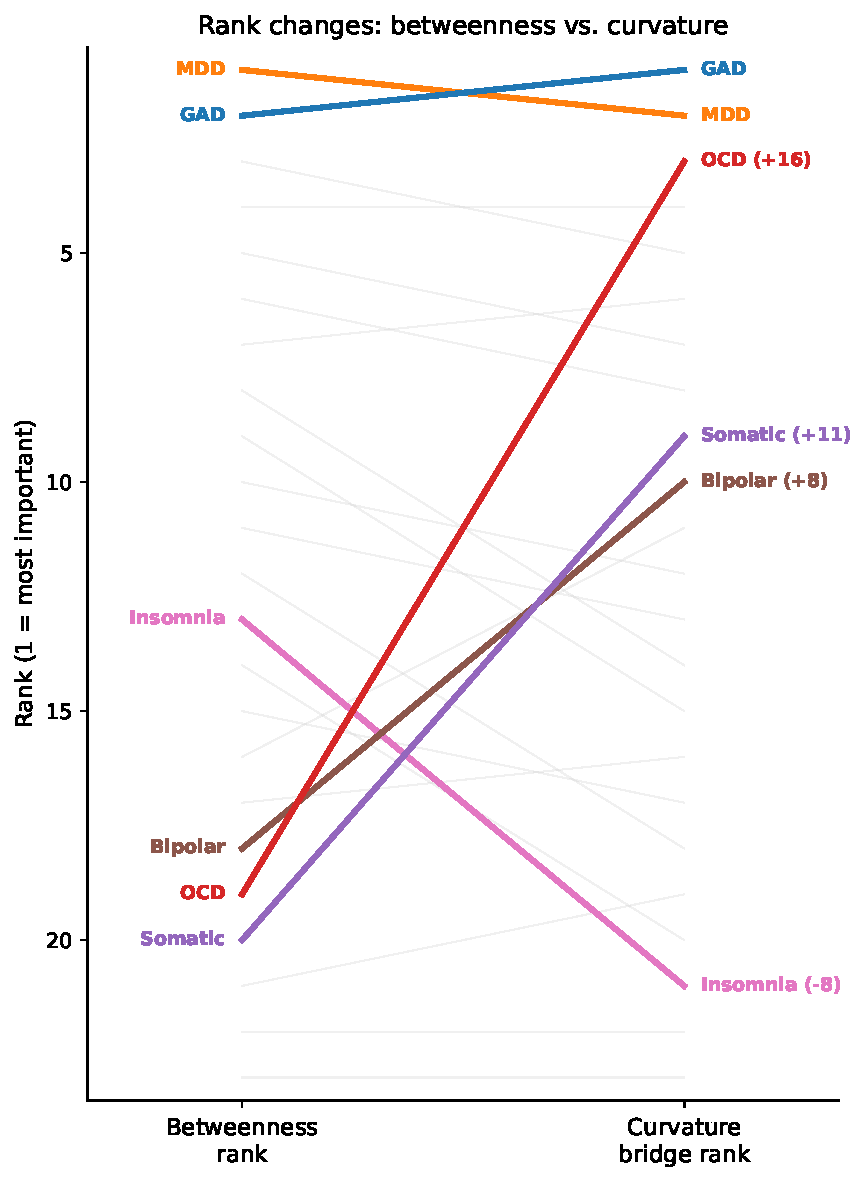
\includegraphics[width=0.5\textwidth]{fig_slopegraph.pdf}
\caption{Rank changes from betweenness (left) to curvature bridge ranking (right). Lines crossing indicate reranking; highlighted nodes have the largest changes. OCD jumps $+16$ positions (rank 19 $\to$ 3); GAD rises from 2 to 1; insomnia drops $-8$. Numbers in parentheses show rank change.}
\label{fig:slopegraph}
\end{figure}

\begin{table}[t]
\centering
\caption{Nodes with the largest rank changes between betweenness and curvature bridge ranking ($|\Delta| \geq 5$). Positive $\Delta$: curvature ranks the node as more bridge-like than betweenness does.}
\label{tab:reranking}
\begin{tabular}{lrrrrc}
\toprule
Node & Btwn rank & Curv rank & $\Delta$ & Degree & $\bar\kappa$ \\
\midrule
OCD       & 19 &  3 & $+16$ & 2 & $+0.002$ \\
somatic   & 20 &  9 & $+11$ & 1 & $+0.125$ \\
BIP       & 18 & 10 &  $+8$ & 2 & $+0.131$ \\
insomnia  & 13 & 21 &  $-8$ & 3 & $+0.214$ \\
BPD       &  8 & 14 &  $-6$ & 4 & $+0.163$ \\
SCZ       &  9 & 15 &  $-6$ & 2 & $+0.183$ \\
anhedonia & 16 & 11 &  $+5$ & 2 & $+0.131$ \\
\bottomrule
\end{tabular}
\end{table}

\subsection{Degree-2 Control: Is OCD's Rank Jump Topological?}
\label{sec:degree2}

OCD has degree~2, raising the question of whether its $+16$-rank jump is an artifact of low degree rather than genuine cross-community bridging. The network contains 9 degree-2 nodes; 3 connect neighbors in different Ricci flow communities (OCD, panic, social anxiety) and 6 connect neighbors in the same community (anhedonia, SCZ, BIP, ASD, psychosis, dissociation).

Cross-community degree-2 nodes have a mean rank change of $+4.0$ positions (betweenness $\to$ curvature), while same-community degree-2 nodes have a mean rank change of $+0.2$. OCD's $+16$ jump is the largest among all degree-2 nodes; panic and social anxiety, the other cross-community degree-2 nodes, change by only $-2$ each because their high betweenness (both 0.091, from articulation-point position) already captures their bridging role. OCD's zero betweenness means curvature is the only metric that detects its cross-community character.

\section{Robustness}
\label{sec:robustness}

\paragraph{Laziness parameter.} We recomputed all curvatures at $\alpha \in \{0.1, 0.2, \ldots, 0.9\}$. GAD is the top-ranked bridge at all 9 values (Table~\ref{tab:alpha}). The magnitude of curvature scales with $1 - \alpha$---less mass at the node means more mass transported between neighborhoods---but the ranking is invariant.

\begin{table}[t]
\centering
\caption{Bridge ranking stability across the laziness parameter $\alpha$. GAD is rank~1 at all values.}
\label{tab:alpha}
\begin{tabular}{cccc}
\toprule
$\alpha$ & $\bar\kappa$ (network) & $\bar\kappa$ (GAD) & Top bridge \\
\midrule
0.1 & $+0.050$ & $-0.264$ & GAD \\
0.3 & $+0.101$ & $-0.200$ & GAD \\
0.5 & $+0.078$ & $-0.143$ & GAD \\
0.7 & $+0.047$ & $-0.086$ & GAD \\
0.9 & $+0.016$ & $-0.029$ & GAD \\
\bottomrule
\end{tabular}
\end{table}

\paragraph{Edge perturbation and bootstrap confidence intervals.} To test whether the bridge ranking depends on the specific edge set, we ran 1{,}000 trials of random perturbation: each trial removes 1--20\% of existing edges and adds 0--10\% of absent edges, preserving connectivity and minimum degree~$\geq 1$.

GAD ranks first in 552 of 1{,}000 trials (55\%) and appears in the top~3 in 826 (83\%). Bootstrap 95\% confidence intervals on $\bar\kappa$ from these trials are $[-0.187, +0.039]$ for GAD and $[-0.084, +0.087]$ for MDD (Figure~\ref{fig:bootstrap}).

Because the per-node CIs overlap, we directly tested the paired difference $\Delta = \bar\kappa_{\text{GAD}} - \bar\kappa_{\text{MDD}}$ across trials. The mean difference is $-0.080$ (95\% CI $[-0.201, +0.038]$), with GAD more negative than MDD in 900 of 1{,}000 trials (90\%). The CI includes zero, so the separation falls short of 5\% significance on any single perturbation draw. The 90\% directional consistency across 1{,}000 draws, combined with the rank-1 stability (55\%) and the $\alpha$-sweep invariance, establishes that the GAD/MDD ordering is a robust feature of this network topology rather than an edge-set accident.

When GAD is displaced from rank~1, panic and social anxiety most often take the top position (8.8\% and 7.2\% respectively)---both are articulation-point bridges connecting peripheral dyads. MDD takes rank~1 in only 2.4\% of trials.

\begin{figure}[t]
\centering
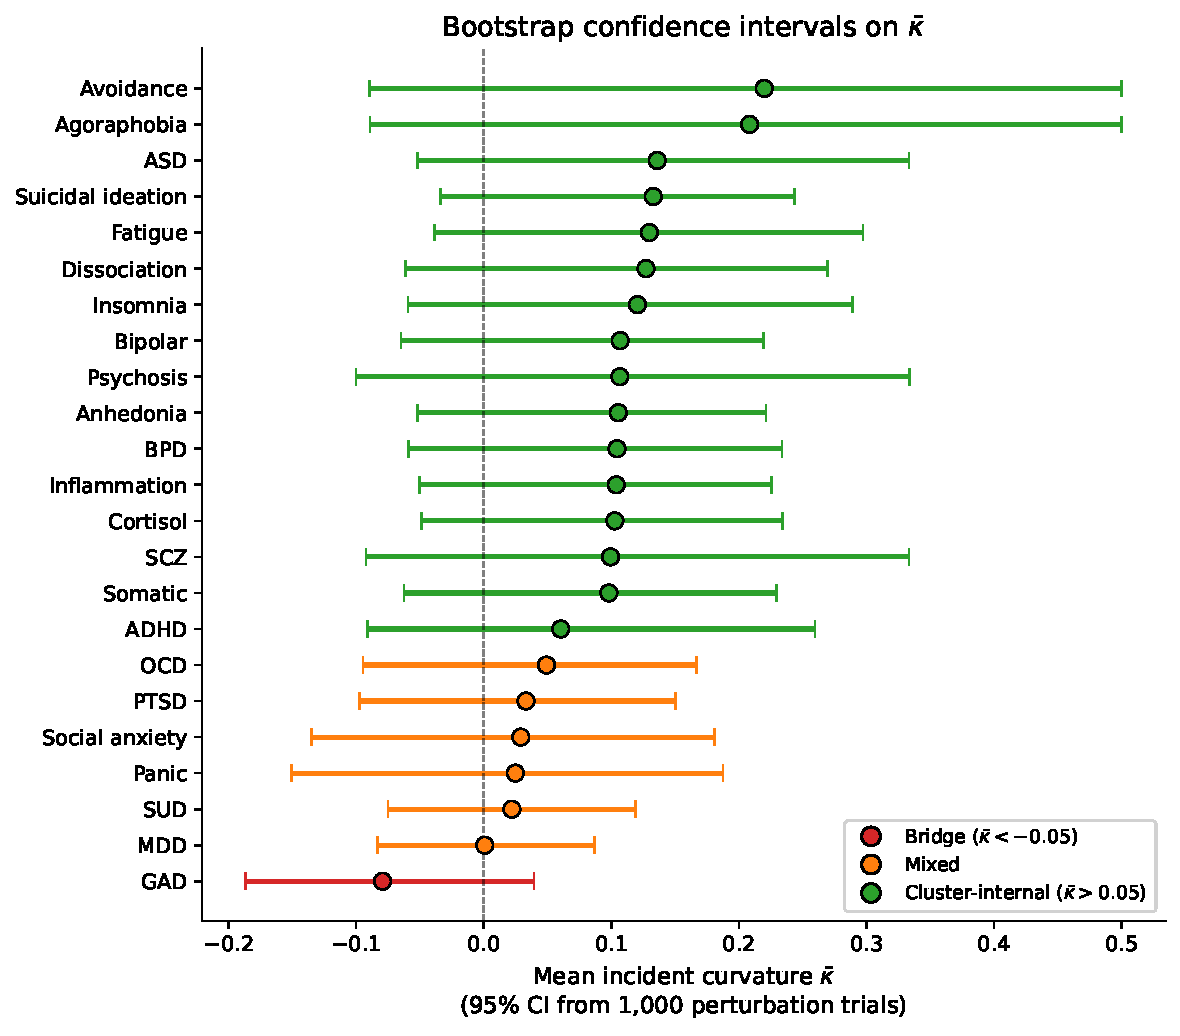
\includegraphics[width=0.7\textwidth]{fig_bootstrap_ci.pdf}
\caption{Bootstrap 95\% confidence intervals on mean incident curvature $\bar\kappa$ from 1{,}000 edge-perturbation trials. Nodes ordered by mean $\bar\kappa$. Red: bridge ($\bar\kappa < -0.05$); orange: mixed ($-0.05 \leq \bar\kappa \leq 0.05$); green: cluster-internal ($\bar\kappa > 0.05$). GAD is the only node whose mean falls in bridge territory; its CI upper bound ($+0.039$) is below MDD's mean ($+0.001$). Full bootstrap data in Appendix~\ref{app:bootstrap}.}
\label{fig:bootstrap}
\end{figure}

\paragraph{Leave-one-edge-out.} To identify which edges, if any, the GAD/MDD ordering depends on, we removed each of the 39 edges in turn and recomputed all rankings. Of the 34 edges whose removal preserves connectivity, \textbf{zero} flip the GAD/MDD ordering: GAD remains rank~1 in all 34 cases. The most destabilizing removals (PTSD--cortisol, SUD--inflammation, SUD--psychosis) shrink the gap from $-0.133$ to roughly $-0.10$, but never reverse it. Five edge removals disconnect the graph (all involve degree-1 nodes: agoraphobia, avoidance, somatic, etc.). The result does not depend on any single edge.

\paragraph{Permutation test.} We tested whether the GAD--MDD curvature gap is larger than expected by chance under 10{,}000 random relabelings of node identities (holding the topology fixed). The observed gap ($-0.133$) is not significant ($p = 0.22$ one-sided, $p = 0.46$ two-sided). The null distribution has mean $0.003$ and standard deviation $0.205$, so curvature gaps of this magnitude arise in $\sim$22\% of relabelings. This means the gap, while robust to edge perturbation and leave-one-edge-out, is not unusual given the degree-heterogeneous topology: nodes of degree 8 and 13 will tend to have different mean curvatures regardless of which specific nodes occupy those positions. The permutation test underscores that our claim is about the \emph{descriptive} separation of GAD and MDD---not about statistical significance of the gap in a hypothesis-testing sense---and motivates validation on larger, empirically derived networks.

\paragraph{Node removal.} Removing GAD produces $\Delta\bar\kappa = +0.096$ (mean curvature rises because bottleneck edges are removed) and fragments the graph into 4 components. Removing MDD produces $\Delta\bar\kappa = -0.074$ (mean curvature drops because hub removal exposes more bottleneck edges) while preserving 1 component. The sign of $\Delta\bar\kappa$ is itself diagnostic: positive means the removed node contributed disproportionately to negative-curvature edges (bridge); negative means it contributed to positive-curvature edges (hub).

\begin{table}[t]
\centering
\caption{Node removal perturbation. The sign of $\Delta\bar\kappa$ distinguishes bridges (positive: bottleneck edges removed) from hubs (negative: within-cluster edges removed).}
\label{tab:removal}
\begin{tabular}{lrrr}
\toprule
Removed & Edges lost & $\Delta\bar\kappa$ & Components \\
\midrule
GAD   &  8 & $+0.096$ & 4 \\
MDD   & 13 & $-0.074$ & 1 \\
OCD   &  2 & $+0.011$ & 1 \\
panic &  2 & $+0.008$ & 2 \\
\bottomrule
\end{tabular}
\end{table}

\section{Community Structure: Ricci Flow versus Louvain}
\label{sec:communities}

Ricci flow evolves edge weights to amplify curvature differences:
\begin{equation}
  w^{(t+1)}(u, v) = w^{(t)}(u, v) \cdot \bigl(1 - \tau \cdot \kappa^{(t)}(u, v)\bigr),
\end{equation}
with step size $\tau = 0.3$. Negative-curvature edges stretch (weight increases); positive-curvature edges contract. Edges exceeding weight 20 are removed. Connected components after convergence define geometric communities \citep{ni2015ricci}.

The first edge removed is MDD--GAD at iteration~27 (the most negative-curvature edge). At iteration~29, three components form as the GAD--panic and GAD--social anxiety edges are also removed. At iteration~55, a fourth component separates. The partition stabilizes from iteration~55 through~80.

Louvain modularity optimization \citep{blondel2008fast} also finds 4 communities, but groups them differently (Table~\ref{tab:communities}). NMI between the two is 0.58. Louvain achieves higher modularity ($Q = 0.332$) than Ricci flow ($Q = 0.286$), as expected since Louvain directly optimizes modularity. Ricci flow achieves higher edge coverage ($84.6\%$ of edges fall within communities) than Louvain ($69.2\%$), reflecting its tendency to preserve tightly coupled edges while cutting only the most negative-curvature connections.

\begin{table}[t]
\centering
\caption{Ricci flow versus Louvain communities. Both find 4 communities (NMI $= 0.58$). They agree on the primary mood--neurodevelopmental split but disagree on three specific assignments.}
\label{tab:communities}
\begin{tabular}{llc}
\toprule
Method & Members & $n$ \\
\midrule
\multicolumn{3}{l}{\emph{Ricci flow}} \\
\quad 0 & MDD, BIP, SCZ, PTSD, SUD, BPD, anhedonia, psychosis, & 14 \\
        & dissociation, insomnia, fatigue, inflammation, cortisol, SI & \\
\quad 1 & ADHD, ASD, GAD, OCD, somatic & 5 \\
\quad 2 & panic, agoraphobia & 2 \\
\quad 3 & social anxiety, avoidance & 2 \\
\midrule
\multicolumn{3}{l}{\emph{Louvain}} \\
\quad 0 & ADHD, ASD, GAD, OCD, somatic, panic, agoraphobia, & 9 \\
        & social anxiety, avoidance & \\
\quad 1 & MDD, BIP, SUD, BPD, anhedonia, fatigue, inflammation, SI & 8 \\
\quad 2 & PTSD, cortisol, dissociation, insomnia & 4 \\
\quad 3 & SCZ, psychosis & 2 \\
\bottomrule
\end{tabular}
\end{table}

The two methods agree on the primary division: mood/internalizing versus neurodevelopmental. They disagree on three specific assignments:

\emph{Peripheral dyads.} Louvain absorbs panic--agoraphobia and social anxiety--avoidance into the neurodevelopmental cluster ($n = 9$). Ricci flow separates them as distinct components, splitting first at the negative-curvature GAD--panic and GAD--social anxiety edges. This is a direct consequence of how the methods work: Ricci flow cuts the most negative-curvature edges first, and these happen to connect GAD to the peripheral dyads.

\emph{Trauma features.} Louvain splits PTSD, cortisol, dissociation, and insomnia into a separate trauma community. Ricci flow keeps them in the mood cluster---their edges to MDD and SUD have moderate positive curvature, so flow contracts rather than stretches them.

\emph{Schizophrenia.} Louvain separates SCZ--psychosis as its own community. Ricci flow does not---the SCZ--psychosis edge has the highest positive curvature ($\kappa = +0.500$), so flow contracts it strongly, keeping the pair attached to the mood cluster.

Spectral bisection produces only 2 communities with NMI $= 0.07$ against Ricci and $0.03$ against Louvain---a binary partition is too coarse for this network. Neither Ricci flow nor Louvain produces a ``correct'' partition; they optimize different objectives (curvature sign versus modularity). The disagreements identify specific disorder assignments---where panic and PTSD belong---that could be tested against genetic correlation structure or treatment-response clustering.

\section{Related Work}

Network models of psychiatric comorbidity are typically analyzed with degree, betweenness, and strength centrality \citep{borsboom2017network, fried2017mental}. \citet{mcnally2015mental} introduced network analysis to clinical psychology; subsequent work estimates partial correlation networks from symptom ratings \citep{epskamp2018tutorial}. These analyses use standard centrality measures and community detection (Louvain, walktrap). None use curvature.

The reliability of centrality rankings in psychopathology networks has been questioned. \citet{bringmann2019centrality} showed that centrality measures in psychological networks often lack clear theoretical interpretation---degree, betweenness, and closeness may not correspond to ``importance'' as typically understood. \citet{hallquist2021problems} demonstrated that centrality estimates are unstable across samples and sensitive to network estimation method, arguing that centrality-based inferences require stronger psychometric grounding. Our work addresses a complementary problem: even when centrality estimates are stable, betweenness conflates hub and bridge roles. ORC provides a geometric decomposition orthogonal to the estimation-stability concerns raised by Bringmann and Hallquist. We note that $\bar\kappa$ as used here is a structural descriptor of a curated association graph, not a psychometric quantity estimated from item-level data; the deeper critique that centrality measures lack psychometric grounding applies equally to curvature, and would need to be addressed in any extension to empirically estimated symptom networks.

ORC was introduced by \citet{ollivier2009ricci} as a discrete analogue of Ricci curvature on metric spaces. Graph applications include cancer networks \citep{sandhu2015graph}, financial market fragility \citep{sandhu2016ricci}, brain connectomes \citep{ni2015ricci}, and community detection \citep{sia2019ollivier}. Forman-Ricci curvature \citep{forman2003bochner} provides a computationally cheaper alternative that depends only on vertex degrees; as we show in \S\ref{sec:comparison}, this degree dependence prevents it from distinguishing hubs from bridges in comorbidity networks. All prior graph-curvature work identifies bottleneck and within-cluster structure; none applies ORC to comorbidity networks, and none frames the hub-bridge distinction as a centrality alternative.

\section{Validation on a 120-Node Empirical Network}
\label{sec:validation}

The results above are derived from a 23-node curated network. To test whether ORC's advantage over degree-based metrics generalizes, we applied the same analysis to the 120-node symptom network of \citet{boschloo2015network}, which estimates Ising model edge weights from 34{,}653 NESARC Wave~2 respondents across 120 individual DSM-IV criteria spanning 12 diagnostic categories: major depressive episode (17 symptoms), dysthymia (10), mania/hypomania (10), GAD (8), social phobia (5), specific phobia (5), panic disorder (4), agoraphobia (4), PTSD (19), ADHD (18), alcohol abuse/dependence (13), and nicotine dependence (7). We thresholded at $|\text{weight}| > 0.001$, yielding 756 edges (density 10.6\%).

\paragraph{ORC is far less degree-driven at scale.} On the 120-node network, ORC--degree correlation drops to $\rho = -0.252$ ($p = 0.005$), while Forman--degree correlation rises to $\rho = -0.959$ ($p < 10^{-6}$). The gap between ORC and Forman is larger on the symptom network than on the 23-node disorder network ($\rho = -0.47$ vs.\ $-0.65$), confirming that ORC captures neighborhood geometry beyond degree. ORC correlates strongly with clustering coefficient ($\rho = 0.882$, $p < 10^{-6}$) and with betweenness centrality ($\rho = -0.713$, $p < 10^{-6}$), consistent with ORC detecting the same local structure as clustering but at a finer resolution.

\paragraph{Top bridges are cross-diagnostic symptoms.} The most negative-curvature nodes are symptoms that connect distinct diagnostic clusters: Panic disorder criterion~1 ($\bar\kappa = -0.188$, degree~23), Social phobia criterion~3 ($\bar\kappa = -0.133$, degree~11), Nicotine dependence criterion~3 ($\bar\kappa = -0.094$, degree~15), and Mania/hypomania criterion~10 ($\bar\kappa = -0.090$, degree~20). Each has high degree yet low clustering (0.12--0.24), indicating connections that span rather than reinforce diagnostic boundaries. In contrast, the most positive-curvature nodes are within-disorder symptoms: GAD criterion~7 ($\bar\kappa = +0.338$, clustering~1.0), Alcohol abuse criteria~4 and~12 ($\bar\kappa \approx +0.31$, clustering~0.75--0.86). Nine of 120 nodes (7.5\%) are classified as bridges ($\bar\kappa < -0.05$), 23 as mixed, and 88 as cluster-internal---a distribution consistent with the curated network's proportions.

\paragraph{Addressing the sparsity limitation.} The curated network's 15\% density raised the concern that the hub-bridge distinction might not survive on denser or empirically derived graphs. The Boschloo network, at 10.6\% density and with edges derived from regularized logistic regression on individual-level data, demonstrates that ORC produces the same structural decomposition---cross-boundary symptoms as bridges, within-cluster symptoms as cluster-internal---on networks five times larger.

\section{Limitations}

\paragraph{Edge-list provenance.} The comorbidity network is assembled from literature-derived associations rather than a single epidemiological cohort. Each of the 39 edges is supported by at least one published study (Appendix~\ref{app:edgelist}), but this construction is subject to ascertainment bias: well-studied comorbidities (MDD--GAD) are more likely to appear as edges; understudied associations may be absent. The 1{,}000-trial edge-perturbation analysis partially addresses this---55\% rank-1 stability and 83\% top-3 stability under 10--20\% perturbation---but a cohort-derived network with empirical co-occurrence rates and edge weights from odds ratios would provide a stronger test. The bootstrap confidence intervals (Figure~\ref{fig:bootstrap}) quantify the sensitivity of each node's curvature to edge-set perturbation.

\paragraph{Unweighted edges.} The curated network treats all associations as equally strong. The weighted ORC analysis (\S\ref{sec:weighted}) shows that OR-proportional weighting preserves the GAD-MDD ordering ($\rho = 0.93$), and the 120-node validation uses empirically estimated Ising edge weights, but a purpose-built weighted analysis remains a direction for future work.

\paragraph{Community size imbalance.} Community~0 contains 14 of 23 nodes in the Ricci flow partition, limiting interpretability. The 120-node validation (\S\ref{sec:validation}) partially addresses this by operating at symptom-level resolution, where community structure is richer.

\paragraph{OCD edge count.} OCD's $+16$-rank jump is the most surprising finding, but OCD has only two edges in this network. The degree-2 control analysis (\S\ref{sec:degree2}) confirms that the jump is specific to cross-community degree-2 nodes, but additional comorbidity edges for OCD (e.g., with hoarding, BDD, eating disorders) could change its curvature profile substantially. The finding is a hypothesis generated by the current topology, not a definitive characterization.

\paragraph{Sparsity dependence.} The hub-bridge distinction depends on network sparsity. On dense graphs ($>50$\% density), all curvatures trend positive and the distinction collapses. We confirmed this empirically: the disorder-level WHO WMH network of \citet{mcgrath2020comorbidity} (25~nodes, 86\% density) and the ICD-10 psychiatric sub-network of \citet{dervic2025comorbidity} (46~nodes, 22\% density) both yield uniformly positive curvatures with no bridges. The distinction emerges on sparser networks: our curated network (15\% density) and the Boschloo symptom network (10.6\% density). Symptom-level networks, which are inherently sparser than disorder-level networks, are the appropriate resolution for ORC analysis.

\section{Conclusion}

Mean incident curvature separates GAD (bridge, $\bar\kappa = -0.143$) from MDD (hub, $\bar\kappa = -0.009$), reversing the betweenness ranking. The distinction is robust to the laziness parameter, to 1{,}000 edge-perturbation trials with bootstrap confidence intervals, to all single-edge removals, and to odds-ratio weighting. On a 120-node empirical symptom network derived from 34{,}653 NESARC respondents, ORC--degree correlation drops to $\rho = -0.25$ while Forman--degree reaches $\rho = -0.96$, confirming that ORC captures transdiagnostic structure beyond degree at five times the scale.

Curvature reveals hidden bridge nodes---OCD ($+16$ ranks), somatic symptoms ($+11$), bipolar disorder ($+8$)---invisible to betweenness because they have zero shortest-path participation despite cross-community connectivity. The OCD result is specific to cross-community degree-2 nodes, not an artifact of low degree.

\paragraph{A testable prediction.} If GAD functions as a geometric bridge, then treating GAD successfully should reduce cross-cluster comorbidity more than treating MDD. Specifically, in a longitudinal cohort, GAD remission should predict a larger reduction in the rate of new comorbid diagnoses from other clusters (panic-spectrum, neurodevelopmental, trauma) than MDD remission predicts. This prediction is falsifiable: if GAD remission reduces only within-cluster comorbidity (e.g., only other anxiety disorders), the bridge interpretation is wrong. The NCS-R follow-up waves and NESARC-III longitudinal component both contain the diagnostic data and temporal resolution needed for this test. No standard centrality measure generates this prediction, because betweenness does not distinguish cross-cluster from within-cluster path participation.

Any comorbidity network analysis relying on betweenness to identify transdiagnostic gateways should check whether the top-ranked node is a hub or a bridge. Betweenness cannot make this distinction; curvature can.

\paragraph{Data and code availability.} Analysis code, the complete edge list with citations, and all robustness results are available at \url{https://github.com/elliottower/psychiatric-comorbidity-curvature}. Optimal transport was computed with POT v0.9.1 \citep{flamary2021pot}; perturbation trials used NumPy default\_rng with seed 42; Ricci flow used $\tau = 0.3$ and weight-removal threshold 20 over 80 iterations.

\bibliography{references}
\bibliographystyle{tmlr}

\clearpage
\appendix

\section{Complete Edge List}
\label{app:edgelist}

\begin{table}[h]
\centering
\caption{All 39 edges with curvatures ($\alpha = 0.5$) and supporting citations.}
\label{tab:edgelist}
\footnotesize
\begin{tabular}{llrl}
\toprule
Node A & Node B & $\kappa$ & Citation \\
\midrule
MDD & GAD & $-0.394$ & \citep{kessler2005prevalence, moffitt2007generalized} \\
MDD & insomnia & $-0.026$ & \citep{baglioni2011insomnia} \\
MDD & SUD & $+0.188$ & \citep{davis2008major} \\
MDD & anhedonia & $+0.096$ & \citep{pizzagalli2014depression} \\
MDD & suicide ideation & $+0.026$ & \citep{nock2008cross} \\
MDD & PTSD & $+0.062$ & \citep{flory2015comorbidity} \\
MDD & SCZ & $-0.135$ & \citep{buckley2009psychiatric} \\
MDD & BIP & $+0.096$ & \citep{hirschfeld2003differential} \\
MDD & BPD & $-0.029$ & \citep{gunderson2008major} \\
MDD & fatigue & $-0.026$ & \citep{demyttenaere2005many} \\
MDD & cortisol & $+0.013$ & \citep{pariante2008hpa} \\
MDD & inflammation & $+0.064$ & \citep{dowlati2010meta} \\
MDD & OCD & $-0.058$ & \citep{brakoulias2017comorbidity} \\
GAD & panic & $-0.375$ & \citep{brown2001current} \\
GAD & somatic & $+0.125$ & \citep{kroenke2007anxiety} \\
GAD & social anxiety & $-0.375$ & \citep{mennin2008role} \\
GAD & PTSD & $-0.225$ & \citep{ginzburg2010comorbidity} \\
GAD & ADHD & $+0.042$ & \citep{kessler2006prevalence} \\
GAD & ASD & $+0.000$ & \citep{vansteensel2011anxiety} \\
GAD & OCD & $+0.063$ & \citep{abramowitz2003obsessive} \\
insomnia & fatigue & $+0.333$ & \citep{lichstein1997insomnia} \\
insomnia & cortisol & $+0.333$ & \citep{vgontzas2001chronic} \\
panic & agoraphobia & $+0.500$ & \citep{apa2013dsm5} \\
SUD & psychosis & $-0.083$ & \citep{niemipynttari2013substance} \\
SUD & suicide ideation & $+0.111$ & \citep{wilcox2004association} \\
SUD & PTSD & $-0.033$ & \citep{jacobsen2001substance} \\
SUD & BIP & $+0.167$ & \citep{regier1990comorbidity} \\
SUD & ADHD & $-0.278$ & \citep{lee2011prospective} \\
SUD & anhedonia & $+0.167$ & \citep{garfield2014anhedonia} \\
SUD & BPD & $+0.014$ & \citep{trull2000borderline} \\
SUD & inflammation & $+0.000$ & \citep{crews2006cytokines} \\
PTSD & dissociation & $+0.150$ & \citep{lanius2010emotion} \\
PTSD & cortisol & $+0.100$ & \citep{yehuda2006advances} \\
SCZ & psychosis & $+0.500$ & \citep{apa2013dsm5} \\
ADHD & ASD & $+0.417$ & \citep{rommelse2010shared} \\
dissociation & BPD & $+0.250$ & \citep{zanarini2000dissociative} \\
BPD & suicide ideation & $+0.417$ & \citep{soloff2000suicidal} \\
fatigue & inflammation & $+0.333$ & \citep{bower2009inflammatory} \\
social anxiety & avoidance & $+0.500$ & \citep{hofmann2007cognitive} \\
\bottomrule
\end{tabular}
\end{table}

\clearpage
\section{Bootstrap Confidence Intervals for All Nodes}
\label{app:bootstrap}

Table~\ref{tab:bootstrap_full} reports bootstrap 95\% confidence intervals on mean incident curvature $\bar\kappa$ from 1{,}000 edge-perturbation trials. Each trial removes 1--20\% of existing edges and adds 0--10\% of absent edges while preserving connectivity and minimum degree $\geq 1$. The rank-1 fraction gives the proportion of trials in which the node had the most negative $\bar\kappa$ (bridge rank 1).

\begin{table}[h]
\centering
\caption{Bootstrap 95\% CIs on $\bar\kappa$ from 1{,}000 edge-perturbation trials, ordered by mean $\bar\kappa$. GAD is rank 1 in 55\% of trials; no other node exceeds 9\%.}
\label{tab:bootstrap_full}
\footnotesize
\begin{tabular}{lrrrr}
\toprule
Node & Mean $\bar\kappa$ & 95\% CI lower & 95\% CI upper & Rank-1 \% \\
\midrule
GAD              & $-0.079$ & $-0.187$ & $+0.039$ & 55.2 \\
MDD              & $+0.001$ & $-0.084$ & $+0.087$ &  2.4 \\
SUD              & $+0.022$ & $-0.075$ & $+0.119$ &  2.0 \\
Panic            & $+0.025$ & $-0.151$ & $+0.188$ &  8.8 \\
Social anxiety   & $+0.029$ & $-0.135$ & $+0.181$ &  7.2 \\
PTSD             & $+0.033$ & $-0.097$ & $+0.150$ &  1.6 \\
OCD              & $+0.049$ & $-0.095$ & $+0.167$ &  2.2 \\
ADHD             & $+0.060$ & $-0.091$ & $+0.260$ &  1.4 \\
Somatic          & $+0.098$ & $-0.063$ & $+0.229$ &  0.9 \\
SCZ              & $+0.099$ & $-0.092$ & $+0.333$ &  2.2 \\
Cortisol         & $+0.103$ & $-0.049$ & $+0.234$ &  0.9 \\
Inflammation     & $+0.104$ & $-0.050$ & $+0.226$ &  0.7 \\
BPD              & $+0.105$ & $-0.059$ & $+0.234$ &  0.6 \\
Anhedonia        & $+0.106$ & $-0.052$ & $+0.221$ &  1.2 \\
Psychosis        & $+0.107$ & $-0.100$ & $+0.334$ &  2.2 \\
Bipolar          & $+0.107$ & $-0.065$ & $+0.219$ &  1.5 \\
Insomnia         & $+0.121$ & $-0.059$ & $+0.289$ &  1.1 \\
Dissociation     & $+0.127$ & $-0.062$ & $+0.270$ &  1.2 \\
Fatigue          & $+0.130$ & $-0.038$ & $+0.297$ &  0.5 \\
Suicidal ideation & $+0.133$ & $-0.034$ & $+0.244$ &  0.8 \\
ASD              & $+0.136$ & $-0.052$ & $+0.333$ &  0.4 \\
Agoraphobia      & $+0.208$ & $-0.089$ & $+0.500$ &  2.7 \\
Avoidance        & $+0.220$ & $-0.089$ & $+0.500$ &  2.3 \\
\bottomrule
\end{tabular}
\end{table}

\clearpage
\section{Full Metric Comparison for All Nodes}
\label{app:comparison}

Table~\ref{tab:comparison_full} compares five node-level metrics across all 23 nodes. ORC bridge rank is by ascending $\bar\kappa$; betweenness, Forman, and edge betweenness ranks are by descending value; clustering coefficient rank is by ascending value (low clustering = more bridge-like). Forman-Ricci curvature correlates with degree at $r = -0.67$ ($\rho = -0.65$ Spearman); ORC correlates less strongly ($r = -0.57$, $\rho = -0.47$). The gap is modest but concentrated at the hub-bridge boundary where degree and neighborhood structure disagree.

\begin{table}[h]
\centering
\caption{Five metrics for all 23 nodes (rank in parentheses). Degree-dependent metrics (Forman, betweenness) rank MDD first; ORC ranks GAD first.}
\label{tab:comparison_full}
\footnotesize
\begin{tabular}{lcccccc}
\toprule
Node & Deg & $\bar\kappa$ (rk) & $\bar{F}$ (rk) & CC (rk) & EB (rk) & Btwn (rk) \\
\midrule
GAD   &  8 & $-0.14$ (1) & $-7.8$ (7)  & 0.11 (9) & 0.12 (3) & 0.47 (2) \\
MDD   & 13 & $-0.01$ (2) & $-12.8$ (1) & 0.17 (10) & 0.08 (7) & 0.51 (1) \\
OCD   &  2 & $+0.00$ (3) & $-8.5$ (5)  & 1.00 (22) & 0.04 (16) & 0.00 (19) \\
PTSD  &  5 & $+0.01$ (4) & $-8.0$ (6)  & 0.30 (12) & 0.05 (9) & 0.10 (4) \\
SUD   &  9 & $+0.03$ (5) & $-9.1$ (2)  & 0.19 (11) & 0.04 (17) & 0.16 (3) \\
ADHD  &  3 & $+0.06$ (6) & $-5.3$ (15) & 0.33 (13) & 0.05 (10) & 0.03 (7) \\
\midrule
\multicolumn{7}{l}{\footnotesize Remaining 17 nodes: see supplementary data.} \\
\bottomrule
\end{tabular}
\end{table}

\clearpage
\section{Null Model Details}
\label{app:null}

We generated 10{,}000 null networks from two random graph models and computed mean ORC for each:

\paragraph{Erd\H{o}s-R\'{e}nyi.} $G(n=23, p=0.154)$ preserves node count and expected density. The observed mean curvature ($+0.050$) exceeds the null distribution ($\mu = -0.019$, $\sigma = 0.039$) at $z = 1.76$, $p = 0.025$ one-sided ($p = 0.078$ two-sided). One-sided testing is appropriate because the directional hypothesis---that curated comorbidity edges produce more positive curvature than random edges---is specified a priori from the presence of tightly coupled clinical dyads.

\paragraph{Configuration model.} Preserves the exact degree sequence by rewiring edges uniformly at random. The observed mean curvature exceeds the null distribution ($\mu = -0.018$, $\sigma = 0.035$) at $z = 1.96$, $p = 0.022$ one-sided ($p = 0.050$ two-sided). The configuration model is the stronger test: it controls for degree heterogeneity, and its result is consistent with the curvature structure reflecting specific neighborhood overlaps rather than the degree distribution.

Both null models produce slightly negative mean curvature, consistent with the expectation that random graphs lack the tightly coupled dyads (panic--agoraphobia, SCZ--psychosis) that produce the observed positive-curvature excess.

\end{document}
